\chapter{不变定律、四维矢量与场张量}

我们将从一条自然界本可以遵守、却并未遵守的定律开始。它的失效将告诉我们，一条物理定律应当如何书写。同样的检验首先把坐标分量引向普通矢量，继而把普通矢量引向四维矢量，最终把四维矢量引向张量。到末尾时，电场与磁场将不再是彼此分离的对象：它们将共同占据一个反对称张量的六个独立位置。

除非另有说明，我们采用\(c=1\)的单位制，将时空分量排序为\((1,2,3,0)=(x,y,z,t)\)，并使用度规号差\((-,-,-,+)\)。

\section{一条对称性错误的可能定律}

在空间中永久固定一条\(x\)轴和一条\(y\)轴。现在规定：只要两个粒子的\(x\)坐标相同，它们就发生相互作用。这种相互作用可能使它们的运动反向，也可能把它们送往新的方向；其具体动力学并不重要。所提出的触发条件仅仅是
\begin{equation}
  x_1-x_2=0,
\end{equation}
其中下标标记的是粒子，而不是坐标分量。这条规则在数学上并无矛盾。问题在于，它为何在物理上不可信。

\begin{classroomqa}
\audiencequestion{这条规则违反空间均匀性吗？}
\lecturerresponse{不违反。平移原点会使两个坐标改变相同的量，因而\(x_1-x_2\)保持不变。这条规则并未指定任何优先位置。它的缺陷在于各向同性：它挑出了一个优先方向。}
\end{classroomqa}

将坐标轴旋转\(90^\circ\)。原来的\(x\)方向现在称为\(y\)，因此同样的物理事件将被描述为\(y\)坐标相等。在一般角度下，该条件将涉及\(x\)与\(y\)的线性组合。于是，这条定律的形式取决于黑板是如何摆放的。它具有平移不变性，却不具有旋转不变性。

我们通常让物理定律在正交坐标中取最简形式。人们可以使用更一般的坐标，但那样度规和公式就会变得不那么简单。在正交笛卡儿坐标系的类别之内，任何取向都不应享有特权。

修正立即可得。在二维中要求两个坐标都相同；在三维中要求三个坐标都相同：
\begin{equation}
  x_1=x_2,
  \qquad y_1=y_2,
  \qquad z_1=z_2.
\end{equation}
于是，粒子只有在到达同一点时才能相互作用，即使它们沿不同直线趋近该点。

\begin{classroomqa}
\audiencequestion{\(z\)坐标和时间也必须相同吗？}
\lecturerresponse{在三维空间中，\(z\)坐标也必须相同。时间暂时被略去；一旦空间论证完成，它就会被恢复。}
\end{classroomqa}

设\(\boldsymbol r_a\)为粒子\(a\)的位置。三个分量条件变成一个矢量方程，
\begin{equation}
  \boldsymbol r_1-\boldsymbol r_2=\boldsymbol 0.
\end{equation}
一个分量可以在某个旋转后的坐标系中为零，而在另一个坐标系中不为零。整个矢量则不同：如果在一个坐标系中每个分量都为零，那么在每个旋转后的坐标系中每个分量也都为零。同样，如果两个矢量在一个坐标系中相等，那么在对二者都作变换之后，它们仍然相等。

\begin{figure}[H]
\centering
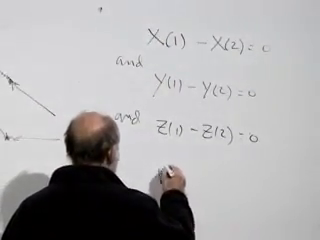
\includegraphics[width=0.78\textwidth]{lecture_06_figure_01.png}
\caption{使碰撞意味着空间重合、而非沿某一优先轴重合的三个坐标等式。}
\lectureframe{00:09:00}
\end{figure}

这就是矢量方程之所以有用的原因。它们的分量会改变，但对象会协调地变换。为完整对象写出的定律，在坐标旋转时能够保持其形式。

\section{时空中的重合}

现在把竖直的空间轴换成时间。一条牛顿式规则可能会说：两次运动变化只有在时间相等时才发生。在牛顿力学中，同时性为所有惯性观察者所共有，因此这样的规则是可能的。在狭义相对论中，它却挑出了一个优先参考系。在一个参考系中同时的事件，在另一个参考系中未必同时。

只要求空间坐标相等也好不到哪里去。一个时空位移可以具有为零的空间分量和一个非零的时间分量，
\begin{equation}
  \Delta X^\mu=(0,0,0,\Delta t),
\end{equation}
而一个助推会把\(\Delta t\)与某个空间分量混合起来。不变性的局域陈述是：两次运动变化发生在同一事件处。因此，一次简单的碰撞要求
\begin{equation}
  X_1^\mu=X_2^\mu,
  \qquad\text{or}\qquad
  X_1^\mu-X_2^\mu=0.
\end{equation}
四个坐标全都相同：粒子在同一时间占据同一地点。

碰撞这个例子给出了书写物理学的一条一般规则。我们可以把所有东西放到一边，令一个完整的四维矢量等于零，或者令一个完整的四维矢量等于另一个。把四维矢量中互不相关的部分彼此等同，本身并不能给出洛伦兹不变的陈述。

\section{助推、旋转与矩阵记法}

四维矢量是这样一种对象：它的变换方式与时空位移的变换方式相同。
为了使这个定义有用，首先回顾坐标本身的变换。对于沿\(x\)方向、速度为\(v\)的助推，
\begin{align}
  x'&=\gamma(x-vt), & y'&=y, & z'&=z,
  & t'&=\gamma(t-vx),                                      \label{eq:l6-boost}
\end{align}
其中
\begin{equation}
  \gamma(v)=\frac{1}{\sqrt{1-v^2}}.
\end{equation}

\begin{classroomqa}
\audiencequestion{在这些公式中，光速是否已被设为1？}
\lecturerresponse{是的。恢复单位后，取\(X^0=ct\)，将\(1-v^2\)替换为\(1-v^2/c^2\)，并在混合的空间--时间项中恢复相应的\(c\)因子。}
\end{classroomqa}

绕\(z\)轴的旋转混合\(x\)和\(y\)，而\(z\)和\(t\)保持不变：
\begin{equation}
\begin{pmatrix}
  x'\\ y'\\ z'\\ t'
\end{pmatrix}
=
\begin{pmatrix}
  \cos\theta & \sin\theta & 0 & 0\\
  -\sin\theta & \cos\theta & 0 & 0\\
  0 & 0 & 1 & 0\\
  0 & 0 & 0 & 1
\end{pmatrix}
\begin{pmatrix}
  x\\ y\\ z\\ t
\end{pmatrix}.
\end{equation}
其中的零值得展示出来：它们明确显示了哪些分量不进入某个给定的变换后坐标。按同样的排列顺序，式~\eqref{eq:l6-boost}中的助推为
\begin{equation}
\begin{pmatrix}
  x'\\ y'\\ z'\\ t'
\end{pmatrix}
=
\begin{pmatrix}
  \gamma & 0 & 0 & -\gamma v\\
  0 & 1 & 0 & 0\\
  0 & 0 & 1 & 0\\
  -\gamma v & 0 & 0 & \gamma
\end{pmatrix}
\begin{pmatrix}
  x\\ y\\ z\\ t
\end{pmatrix}.
\end{equation}

旋转和助推可以通过矩阵乘法复合。要沿与原始\(x\)轴不对齐的方向进行助推，可以先将该方向旋转到\(x\)轴，施加助推，再按需旋转回去。这些初等矩阵的乘积生成更一般的洛伦兹变换。

\begin{classroomqa}
\audiencequestion{先旋转再助推，还是先助推再旋转，这有区别吗？}
\lecturerresponse{有。第一次操作之后，第二次操作所作用的轴已经改变了。两个矩阵乘积不必相等，因此操作的顺序是有关系的。}
\end{classroomqa}

所有这些线性变换可以一次性写成
\begin{equation}
  X'^{\mu}=\Lambda^{\mu}{}_{\nu}X^{\nu}.                  \label{eq:l6-vector-transform}
\end{equation}
重复指标\(\nu\)对\(1,2,3,0\)求和。这不过是矩阵乘法中通常的逐行逐列求和，用指标记号表达出来而已。

\begin{figure}[H]
\centering
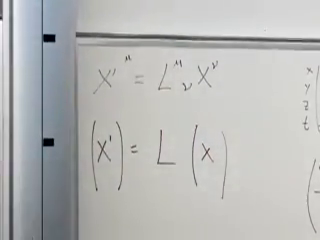
\includegraphics[width=0.78\textwidth]{lecture_06_figure_02.png}
\caption{上述带指标的洛伦兹变换，位于其列矢量形式的开头。}
\lectureframe{00:31:55}
\end{figure}

式~\eqref{eq:l6-vector-transform}也是一般逆变四维矢量的定义。如果\(A^\mu\)是这样一个矢量，那么
\begin{equation}
  A'^{\mu}=\Lambda^{\mu}{}_{\nu}A^{\nu}.
\end{equation}
它的四个分量不必表示位置。使这个对象成为四维矢量的是它的变换规律。

\section{标量、度规与不变量乘积}

在使用更多四维矢量之前，退回到更简单的标量概念是有帮助的。在空间旋转下，指定点处的温度是一个标量，两个指定点之间的距离也是一个标量。它们各自是一个数，与坐标轴的取向无关。人们甚至可以故意提出一个愚蠢的数值断言：以厘米测量的距离等于以华氏度测量的室温。这个断言没有物理深度，但由于两边都是旋转标量，其真假并不取决于坐标轴如何转动。

矢量的分量不是标量。因此我们需要一种系统的方法将它们组合成标量。将一般逆变四维矢量写成
\begin{equation}
  A^\mu=(A^1,A^2,A^3,A^0).
\end{equation}
协变分量用下指标描述同一个几何对象。在我们的号差下，它们通过闵可夫斯基度规得到，
\begin{equation}
  A_\mu=\eta_{\mu\nu}A^\nu,
  \qquad
  \eta_{\mu\nu}=
  \begin{pmatrix}
    -1&0&0&0\\
    0&-1&0&0\\
    0&0&-1&0\\
    0&0&0&1
  \end{pmatrix},                                          \label{eq:l6-metric}
\end{equation}
于是
\begin{equation}
  A_\mu=(-A^1,-A^2,-A^3,A^0).
\end{equation}

\begin{classroomqa}
\audiencequestion{黑板上的两个指标和符号不一致吗？}
\lecturerresponse{是的。所展示的列中的空间分量需要相应的负号，而指标下降方程右边的分量在乘以\(\eta_{\mu\nu}\)之前带有上指标。时间标签是\(0\)，不是\(4\)。}
\end{classroomqa}

\begin{figure}[H]
\centering
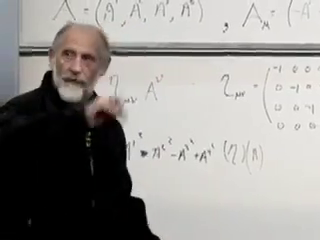
\includegraphics[width=0.8\textwidth]{lecture_06_figure_03.png}
\caption{逆变分量与协变分量、度规矩阵，以及不变量缩并的开头。}
\lectureframe{00:45:00}
\end{figure}

指标下降不是装饰。它把洛伦兹不变模长所需的符号打包在一起：
\begin{align}
  A_\mu A^\mu
  &=-(A^1)^2-(A^2)^2-(A^3)^2+(A^0)^2,                    \label{eq:l6-norm}\\
  X_\mu X^\mu
  &=t^2-x^2-y^2-z^2.
\end{align}
第二个表达式是从原点出发的不变时空间隔。因为\(A^\mu\)的变换方式与\(X^\mu\)相同，所以它的缩并具有同样的不变性。

这种记号还教给我们一条有用的记账规则。重复的求和指标一次出现在上方，一次出现在下方。例如，
\begin{equation}
  A_\mu A^\mu
  =\eta_{\mu\nu}A^\mu A^\nu.
\end{equation}
被求和指标（哑指标）的名称可以改变，而不改变该量。

\begin{classroomqa}
\audiencequestion{这些矢量中的一个是否应被视为行，另一个被视为列，它们的顺序有关系吗？}
\lecturerresponse{就当前的计算而言，把带指标的这些量视为分量，让度规来完成缩并；没有必要把讨论变成行与列的算符代数。这些都是普通数，所以它们的顺序没有关系。非对易算符需要更小心，但这不是这里的主题。}
\end{classroomqa}

同样的构造给出两个不同四维矢量之间的内积，
\begin{equation}
  A\mathbin{\cdot}B=A_\mu B^\mu=A^\mu B_\mu.
\end{equation}
无需写出显式的洛伦兹矩阵即可得到其不变性。由于
\(A+B\) 和 \(A-B\) 是四维矢量，它们的模平方都是
不变的：
\begin{align}
  (A+B)^2&=A^2+B^2+2A\mathbin{\cdot}B,\\
  (A-B)^2&=A^2+B^2-2A\mathbin{\cdot}B.
\end{align}
相减得到
\begin{equation}
  (A+B)^2-(A-B)^2=4A\mathbin{\cdot}B,                    \label{eq:l6-polarization}
\end{equation}
因此 \(A\mathbin{\cdot}B\) 也是不变的。因子四直接来自该展开。\editorialnote{黑板上的论证给出了这个
极化恒等式；写出该因子使口头讲述的相消变得明确无误。}

\begin{figure}[H]
\centering
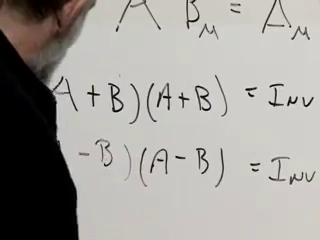
\includegraphics[width=0.8\textwidth]{lecture_06_figure_04.png}
\caption{用于分离不同四维矢量内积的两个不变平方。}
\lectureframe{00:52:20}
\end{figure}

不变量是物理定律的天然组成部分：与孤立的
分量不同，它在不同参考系中取相同的值。

\section{固有速度和四维动量}

考虑粒子世界线上的两个相邻事件。它们的间隔
是无穷小四维矢量
\begin{equation}
  dX^\mu=(dx,dy,dz,dt).
\end{equation}
对于类时世界线，固有时间定义为
\begin{equation}
  d\tau^2=dX_\mu dX^\mu
  =dt^2-dx^2-dy^2-dz^2.                                  \label{eq:l6-proper-time}
\end{equation}
固有四维速度为
\begin{equation}
  U^\mu=\frac{dX^\mu}{d\tau}.                            \label{eq:l6-four-velocity}
\end{equation}
它衡量的是时空位置相对于粒子自身固有时间的变化率，
而不是相对于所选参考系的坐标时间。

尽管 \(U^\mu\) 有四个分量，但只有三个是独立的。将
式~\eqref{eq:l6-proper-time}除以 \(d\tau^2\) 得到
\begin{equation}
  U_\mu U^\mu=1.
\end{equation}
因此四维速度是单位类时矢量。取指向未来的选择
确定了其时间分量的符号。

\begin{classroomqa}
\audiencequestion{在远小于 \(c\) 的速度下，四维速度是否约化为
普通速度？}
\lecturerresponse{它的三个空间分量趋近于普通速度，
而时间分量在 \(c=1\) 单位下趋近于一。该关系通过
应用链式法则并计算 \(dt/d\tau\) 得到。}
\end{classroomqa}

对每个空间分量，
\begin{equation}
  U^i=\frac{dx^i}{d\tau}
     =\frac{dx^i}{dt}\frac{dt}{d\tau}
     =v^i\frac{dt}{d\tau}.
\end{equation}
将式~\eqref{eq:l6-proper-time}除以 \(dt^2\)：
\begin{equation}
  \left(\frac{d\tau}{dt}\right)^2
  =1-v_x^2-v_y^2-v_z^2
  =1-\boldsymbol v^2.
\end{equation}
因此
\begin{equation}
  \frac{dt}{d\tau}=\frac{1}{\sqrt{1-\boldsymbol v^2}}
  =\gamma(\lvert\boldsymbol v\rvert),
\end{equation}
以及
\begin{equation}
  U^\mu=(\gamma v_x,\gamma v_y,\gamma v_z,\gamma).
                                                                  \label{eq:l6-u-components}
\end{equation}

\begin{figure}[H]
\centering
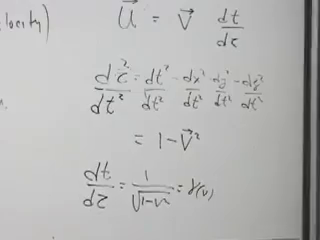
\includegraphics[width=0.8\textwidth]{lecture_06_figure_05.png}
\caption{产生 \(dt/d\tau=\gamma\) 并将固有速度与普通速度联系起来的
固有时间计算。}
\lectureframe{01:02:00}
\end{figure}

\begin{classroomqa}
\audiencequestion{\(dx^2/dt^2\) 是否表示二阶导数，并且
对矢量取平方是否应产生交叉项？}
\lecturerresponse{这里它表示 \((dx/dt)^2\)，即一阶导数的平方。此外，\(\boldsymbol v^2\) 表示欧几里得点积
\(v_x^2+v_y^2+v_z^2\)，而不是形式上的和
\(v_x+v_y+v_z\) 的平方；不存在交叉项。}
\end{classroomqa}

\begin{classroomqa}
\audiencequestion{\(\gamma(v)\) 中的 \(v\) 是两个坐标参考系的
相对速度，还是粒子的速度？}
\lecturerresponse{这里是粒子在所选参考系中的速度。
函数 \(\gamma(v)=1/\sqrt{1-v^2}\) 可以对任意速度求值：在
助推中它按参考系的相对速度求值；在四维速度中它
按粒子速度求值。}
\end{classroomqa}

对于 \(v\ll1\)，\(\gamma\simeq1\)，因此 \(U^\mu\) 的空间分量
趋近于 \(\boldsymbol v\)，而 \(U^0\) 趋近于一。当普通速度
趋近于光速时，\(\gamma\) 以及四维速度的所有非零分量
都无界增长。

\begin{classroomqa}
\audiencequestion{\(U^0\) 难道不应该具有速度的量纲，而不是
接近数字一吗？}
\lecturerresponse{当 \(c\) 被设为一后，量纲就消失了。在
\(X^0=ct\) 下，有
\(U^\mu=(\gamma\boldsymbol v,\gamma c)\)，因此时间分量趋近于
\(c\)，且 \(U_\mu U^\mu=c^2\)。}
\end{classroomqa}

对于静质量为 \(m\) 的粒子，四维动量定义为
\begin{equation}
  P^\mu=mU^\mu.
\end{equation}
在自然单位下，
\begin{equation}
  P^\mu=(\gamma m\boldsymbol v,\gamma m).
\end{equation}
前三个分量在低速下趋近于牛顿动量 \(m\boldsymbol v\)。恢复量纲后得到
\begin{equation}
  P^\mu=(\gamma m\boldsymbol v,E/c),
  \qquad E=\gamma mc^2,
\end{equation}
从而
\begin{equation}
  E=mc^2+\frac{1}{2}m\boldsymbol v^2+O(mv^4/c^2).
\end{equation}
时间分量是以 \(c=1\) 为单位的能量，或者当
四个分量都被赋予动量单位时，是能量除以 \(c\)。

\begin{classroomqa}
\audiencequestion{把普通 \(\boldsymbol v\) 附加第四个分量后，
它本身是四维矢量吗？}
\lecturerresponse{不是。普通三维速度不按
四维矢量变换。因子 \(\gamma\) 和固有时间的定义是
本质性的；四维矢量是 \(U^\mu\)，而不是 \(\boldsymbol v\)。}
\end{classroomqa}

\section{为什么电场和磁场必须混合}

我们现在暂时离开相对论，作一次所谓的短暂休假。从
前爱因斯坦运动方程出发，并追问在它
能在每个惯性系中成立之前必须如何被重新组织。普通加速度是普通速度的
时间导数。它的四维类似物自然是
\begin{equation}
  A^\mu=\frac{dU^\mu}{d\tau}.
\end{equation}
在低速下其空间分量趋近于普通加速度。完整的
相对论方程将推迟讨论；首先考察旧的力定律。

对于在电场和磁场中运动的电荷\(q\)，
\begin{equation}
  \boldsymbol F=m\boldsymbol a
  =q\left(\boldsymbol E+\boldsymbol v\times\boldsymbol B\right).
                                                                  \label{eq:l6-lorentz-force}
\end{equation}
电场项与粒子速度无关，而磁场项则不然。

\begin{figure}[H]
\centering
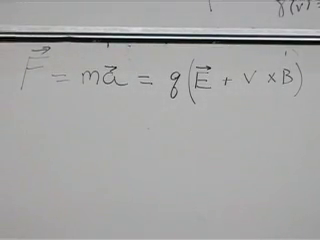
\includegraphics[width=0.8\textwidth]{lecture_06_figure_06.png}
\caption{促使人们将\(\boldsymbol E\)与\(\boldsymbol B\)结合起来的前相对论形式的洛伦兹力定律。}
\lectureframe{01:18:20}
\end{figure}

假设一位观测者看不到电场，但看到了磁场和一个运动电荷。该电荷感受到磁力。然而，在电荷的瞬时静止参考系中，\(\boldsymbol v=0\)，因此式~\eqref{eq:l6-lorentz-force}中的磁场项消失。物理世界线并不会仅仅因为坐标改变就变成惯性的；因此新参考系中的力必须包含电场的贡献。更仔细地说，非零的四维加速度不能通过改变惯性参考系而变换为零，尽管三维加速度及其分量确实会变换。\editorialnote{这一关于四维加速度的陈述是课堂论证的不变形式，并且避免了将普通的三维加速度本身视为参考系不变量。}

因此，电场和磁场必须相互变换。它们合起来有六个分量，所以它们既不是一个标量，也不是一个四维矢量。我们需要一个新的变换对象。

\section{张量：每个指标对应一次变换}

标量可以称为零阶张量；它没有指标。四维矢量是一阶张量；它有一个指标，可取四个值。最简单的二阶例子是乘积
\begin{equation}
  A^\mu B^\nu.
\end{equation}
每个指标有四个值，因此该对象有\(4^2=16\)个分量，可以显示为一个\(4\times4\)阵列。三个矢量的乘积，
\begin{equation}
  A^\mu B^\nu C^\sigma,
\end{equation}
有\(4^3=64\)个分量，是三阶张量。更高阶继续遵循这一模式。名称不如定义该对象的规则重要。

如果
\begin{equation}
  A'^{\mu}=\Lambda^\mu{}_{\nu}A^\nu,
  \qquad
  B'^{\sigma}=\Lambda^\sigma{}_{\tau}B^\tau,
\end{equation}
那么它们的乘积变换为
\begin{equation}
  A'^{\mu}B'^{\sigma}
  =\Lambda^\mu{}_{\nu}\Lambda^\sigma{}_{\tau}
   A^\nu B^\tau.
\end{equation}
这给出了逆变二阶张量的定义定律：
\begin{equation}
  T'^{\mu\sigma}
  =\Lambda^\mu{}_{\nu}\Lambda^\sigma{}_{\tau}T^{\nu\tau}.
                                                                  \label{eq:l6-tensor-transform}
\end{equation}
每个指标对应一个洛伦兹矩阵。重复的\(\nu\)和\(\tau\)被求和；开放的\(\mu\)和\(\sigma\)标记在带撇参考系中正在计算的哪个分量。

\begin{figure}[H]
\centering
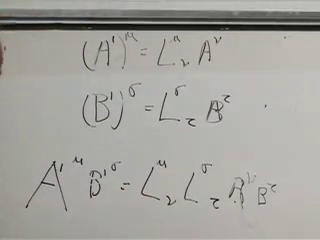
\includegraphics[width=0.82\textwidth]{lecture_06_figure_07.png}
\caption{两个矢量的变换以及由此得到的二阶张量的双矩阵变换定律。}
\lectureframe{01:27:15}
\end{figure}

张量不必是矢量的单一乘积。\(A^\mu B^\nu\)和\(A^\nu B^\mu\)都遵循张量变换定律，它们的和以及任何诸如
\begin{equation}
  A^\mu B^\nu+C^\mu D^\nu.
\end{equation}
这样的和也遵循。定义是变换定律，而不是某种特定的因式分解。三阶张量会获得第三个洛伦兹矩阵，依此类推。

\section{对称张量和反对称张量}

两类二阶张量将特别有用。对称张量满足
\begin{equation}
  T^{\mu\nu}=T^{\nu\mu},
\end{equation}
因此关于对角线反射的矩阵元相等。它的四个对角元和对角线一侧的六个矩阵元决定了其余部分，给出
\begin{equation}
  4+6=10
\end{equation}
个独立分量。

反对称张量满足
\begin{equation}
  T^{\mu\nu}=-T^{\nu\mu}.                                \label{eq:l6-antisymmetry}
\end{equation}
将\(\mu=\nu\)代入式~\eqref{eq:l6-antisymmetry}得到
\(T^{\mu\mu}=-T^{\mu\mu}\)，因此每个对角元都为零。一个三角形半区中的六个矩阵元通过改变符号决定另外六个。因此恰好有六个独立分量。

\begin{figure}[H]
\centering
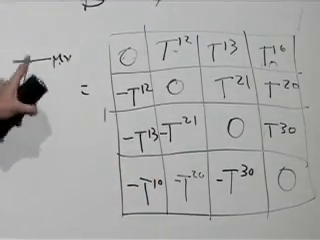
\includegraphics[width=0.82\textwidth]{lecture_06_figure_08.png}
\caption{一个完整的反对称\(4\times4\)阵列：对角线上为零，对角线两侧符号相反。}
\lectureframe{01:34:25}
\end{figure}

这个数目就是线索。三个电场分量和三个磁场分量可以放入一个反对称二阶张量中。

\section{电磁场张量}

让时空标签按\((1,2,3,0)=(x,y,z,t)\)的顺序横跨行和列。黑板上写出的排列是
\begin{equation}
  F_{\mu\nu}=
  \begin{pmatrix}
    0    & -B_3 & B_2  & E_1\\
    B_3  & 0    & -B_1 & E_2\\
    -B_2 & B_1  & 0    & E_3\\
    -E_1 & -E_2 & -E_3 & 0
  \end{pmatrix}.                                         \label{eq:l6-field-tensor}
\end{equation}
纯空间位置包含磁场；带有一个空间指标和一个时间指标的位置包含电场。一旦上三角矩阵元已知，反对称性就给出下三角矩阵元。

\begin{classroomqa}
\audiencequestion{磁场矩阵元是否全为负，并且标签是否对应于\(x,y,z\)？}
\lecturerresponse{上三角空间部分的符号如图所示交替：\(-B_3,+B_2,-B_1\)。标签\(1,2,3\)对应于\(x,y,z\)，而\(0\)标记时间。关于对角线反射会反转每个符号。}
\end{classroomqa}

\begin{figure}[H]
\centering
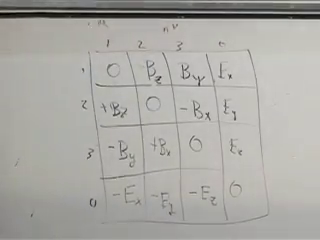
\includegraphics[width=0.82\textwidth]{lecture_06_figure_09.png}
\caption{按讲座中空间分量在前的分量顺序排列的完整电磁场张量。}
\lectureframe{01:41:05}
\end{figure}

按照惯例，这个记号写作\(F_{\mu\nu}\)，而不是一般的\(T_{\mu\nu}\)。讲师推测这个字母可能指法拉第，同时明确表示自己并不了解这一记号的历史。这里重要的是它的反对称性及其六个场分量，而不是关于这个字母的推测。

\begin{classroomqa}
\audiencequestion{矩阵的每个元素是否表示在所示坐标平面内的场的强度？}
\lecturerresponse{它是电磁场张量的一个分量。涉及时间的元素是电分量，而空间--空间元素则编码磁分量。}
\end{classroomqa}

把带有时间指标的列和行隔开。剩下的\(3\times3\)反对称块是磁性的。它的独立元素可以按循环方式记忆：
\begin{equation}
  F_{12}=-B_3,
  \qquad F_{23}=-B_1,
  \qquad F_{31}=-B_2.                                   \label{eq:l6-magnetic-cycle}
\end{equation}
从第一个关系式出发，让每个标号沿\(1\to2\to3\to1\)前进。等价地，
\begin{equation}
  F_{ij}=-\epsilon_{ijk}B_k,
\end{equation}
其中\(\epsilon_{123}=+1\)。\editorialnote{Levi--Civita公式就是黑板上明确展开的循环规则的紧凑标准形式。}

\begin{figure}[H]
\centering
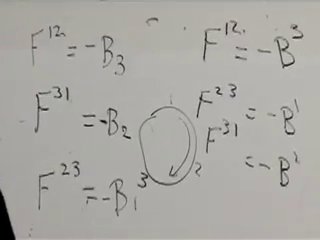
\includegraphics[width=0.82\textwidth]{lecture_06_figure_10.png}
\caption{反对称张量中编码磁场的循环空间分量。}
\lectureframe{01:46:20}
\end{figure}

电场的对应关系更为直接：
\begin{equation}
  E_1=F_{10},
  \qquad E_2=F_{20},
  \qquad E_3=F_{30}.
\end{equation}

因此磁场有两个有用的恒等式。在三维空间中，一个三分量的轴矢量可以与一个\(3\times3\)反对称张量配对。然而在时空中，它只是六分量张量\(F_{\mu\nu}\)的空间部分。这种配对是三维所特有的：一个反对称的\(4\times4\)张量有六个独立分量，不能与四维矢量等同。\editorialnote{在固有旋转下，磁场的行为像矢量；在反射下，更准确地说它是一个轴矢量，或赝矢量。}

这一构造的目的并不是为了数分量而数分量。因为\(F_{\mu\nu}\)按张量变换，洛伦兹助推会自动混合它的电分量和磁分量。在下一讲中，它可以与四维速度和四维加速度结合，用协变运动方程取代式~\eqref{eq:l6-lorentz-force}。

\section{关于爱因斯坦和闵可夫斯基的问题}

最后几分钟从形式体系转向它在历史上的起源。这些回答是作为回忆而非定论性的历史提供的，而这一限定本身就是交流的一部分。

\begin{classroomqa}
\audiencequestion{爱因斯坦是出于概念上的理由在寻求洛伦兹不变的表述，还是被特定的观测所驱动？}
\lecturerresponse{自然定律在每个惯性系中应具有相同形式这一原理是他推理的核心。此外还有关于光的实验证据以及未能探测到通过以太的运动，不过讲师明确表示不确定爱因斯坦知道哪些结果，或者这些结果对他有多大影响。概念上的压力在于，麦克斯韦方程组和洛伦兹力应当服从相对性原理，而这要求电场、磁场和速度分量一起变换。}
\end{classroomqa}

爱因斯坦1905年的表述并没有使用这里所用的紧凑四维矢量记号。它逐分量进行，把必要的\(\gamma\)因子和速度明确写出。闵可夫斯基随后把同样的结构几何化地组织为四维时空。

\begin{classroomqa}
\audiencequestion{爱因斯坦是否抵制闵可夫斯基的时空表述，闵可夫斯基又是在多久之后引入它的？}
\lecturerresponse{课堂上提供的回忆是，爱因斯坦起初并不欢迎四维几何语言，但很快采纳了它的价值。时间被暂定为1905年论文之后大约两年，也许是1907年；讲者强调他是在回忆而不是在确立历史。}
\end{classroomqa}

\begin{classroomqa}
\audiencequestion{闵可夫斯基是数学家还是物理学家，他还贡献了什么，他是否受到洛伦兹或菲茨杰拉德的影响？}
\lecturerresponse{并未声称有确定的答案。数学家和物理学家之间的区分没有被深究，一位听众的更正打断了关于闵可夫斯基其他工作的一段宽泛评论，而可能的影响线索被明确留作不确定。对于这次讨论而言，可靠的一点是闵可夫斯基以四维几何记号对相对性所作的决断性组织。}
\end{classroomqa}

\begin{classroomqa}
\audiencequestion{混合\(\boldsymbol E\)与\(\boldsymbol B\)的变换，在爱因斯坦1905年的工作中就已经出现了吗？}
\lecturerresponse{是的，但当时是逐分量写出的，而不是写成一个场张量方程。课堂上所作的对比是与麦克斯韦的分量方程的比较：内容可以在揭示其共同结构的紧凑记号出现之前就已经存在。闵可夫斯基的贡献在于使这一结构在时空语言中系统化。}
\end{classroomqa}

这就把我们带回了开头所提出的数学要点。分量对于计算是不可或缺的，但当这些分量被认识到是一个变换着的对象的各个部分时，定律才变得可以理解。接下来的任务是用\(F_{\mu\nu}\)把带电粒子的运动方程写成在每个惯性系中都相同的形式。
